\documentclass[12pt,a4paper,italian]{article}


\usepackage[italian]{babel}
\usepackage[latin1]{inputenc}
\usepackage{amsmath}
\usepackage{amsfonts}
\usepackage{amssymb}
\usepackage{color}
\usepackage{xcolor}
\usepackage{hyperref}
\usepackage[all]{hypcap}
\usepackage{ifthen}
\usepackage{wrapfig}
%\author{Piero Bizzotto}
\usepackage[top=2cm,bottom=5cm,left=80pt,right=80pt]{geometry}
\usepackage{graphicx}
\DeclareGraphicsExtensions{.jpg,.png}

\newcommand{\ajax}{AJAXDRAW}
\newcommand{\sito}{\href{http://ajaxdraw.sourceforge.net}{http://ajaxdraw.sourceforge.net}}

\setlength{\parindent}{0pt} %settato indentazione di default 
\setlength{\headheight}{3cm} %settato grandezza header...in altre parole, quanto distanzio il doc dall'intestazione

\usepackage{fancyhdr} %pacchetto per le intestazioni
\pagestyle{fancy} %uso del pacchetto


\fancyhead{} %annulla head di default
\fancyfoot{} %annulla foot di default


\usepackage{lastpage} %setto pg di pgtot a rfoot
     \rfoot{pagina \thepage\ di \pageref{LastPage}}


\lfoot{Versione: \insertversion} %setto versione doc a lfoot
\renewcommand{\footrulewidth}{0.5pt} %ridefinisco il valore della riga di intestazione
\renewcommand{\headrulewidth}{0.5pt} %ridefinisco il valore della riga di pie' di pagina

\newcommand{\insertversion}{0.0} %definisco il nuovo comando per inserire la versione


\lhead{  \begin{Huge} \ajax \end{Huge} \\  %intestazione di sinistra
					%\begin{Large}	Software per il Disegno Grafico\\ in Tecnologie Web \end{Large}  
					\begin{normalsize}\sito \end{normalsize}
			%\\ versione documento: \insertversion\ del \today} %setto l'intestazione sx
		}
\rhead{ %includo logo nell'intestazione dx
	 	
\includegraphics[scale=0.5]{../logo/logo}  
}


%CREAZIONE ELENCHI NUMERATI PERSONALIZZATI
\newcounter{Lcount}
\newcounter{Rcount}
\setcounter{Lcount}{0}
\setcounter{Rcount}{0}

\newenvironment{elenconumerato}[2][ ]
{
  \begin{list}{#1\arabic{Lcount}.}
    {
	\setcounter{Rcount}{\value{Lcount}}
	\setcounter{Lcount}{0} 
	\usecounter{Lcount} 
\addtolength{\leftmargin}{#2pt}
	}
}
{
  \end{list}
 \setcounter{Lcount}{\value{Rcount}}
}

%CREAZIONE ELENCHI PUNTATI
\newenvironment{elencopuntato}[1][]
{
\begin{list}{\textbullet} %\itemindent=#1pt
	{
	\addtolength{\leftmargin}{#1pt}
	}
} 
{
\end{list}
}


\newenvironment{elencodescrittivo}[1][]{\begin{description} \setlength{\itemindent}{#1pt} \addtolength{\leftmargin}{#1pt}} {\end{description}}

\newcommand{\TITOLODOC}{Titolo}

%footer centrale
\cfoot{ \TITOLODOC \\  E-mail:    \href{ mailto:webshape.contact@gmail.com}{ webshape.contact@gmail.com}  }

%INSERIMENTO IMMAGINI
\newcommand{\imagerealsize}[1]{\vspace{20pt} \includegraphics{#1} }
\newcommand{\imageadapted}[1]{\vspace{20pt} \includegraphics[width=1\textwidth]{#1} }

\newcommand{\glosspath}{.\glossario}
\newcommand{\gloss}[1]{\hyperref{\glosspath~\glossario.pdf}{}{#1}{#1}}

\hypersetup{
    %bookmarks=true,         % show bookmarks bar?
    %unicode=false,          % non-Latin characters in Acrobat’s bookmarks
	%pdftoolbar=true,        % show Acrobat’s toolbar?
	%pdfmenubar=true,        % show Acrobat’s menu?
    %pdffitwindow=true,      % page fit to window when opened
    %pdftitle={My title},    % title
    %pdfauthor={Author},     % author
    %pdfsubject={Subject},   % subject of the document
    %pdfnewwindow=true,      % links in new window
    %pdfkeywords={keywords}, % list of keywords
    colorlinks=true,         % false: boxed links; true: colored links
    linkcolor=black,           % color of internal links
    %citecolor=green,        % color of links to bibliography
    %filecolor=magenta,      % color of file links
    urlcolor=teal    % color of external links
%	linktocpage=false;
}


%COLORAZIONE TESTO
\newcommand{\blue}[1]{{\color {blue} #1}} 
\newcommand{\red}[1]{{\color {red} #1}}
\newcommand{\green}[1]{{\color {green} #1}}
\newcommand{\sezione}[1]{\leftskip=0pt \section{#1} \leftskip=18pt}
\newcommand{\subsezione}[1]{\leftskip=18pt \subsection{#1} \leftskip=36pt}
\newcommand{\subsubsezione}[1]{\leftskip=36pt \subsubsection{#1} \leftskip=54pt}
\newcommand{\subsubsecindent}{54}
\newcommand{\subsecindent}{36}
\newcommand{\secindent}{18}
\newcommand{\normindent}{8}
\newcommand{\code}[1]{{\bfseries \texttt{#1}}}
\newcommand{\paragrafo}[1]{\leftskip=36pt \paragraph{#1} \leftskip=54pt}
\newcommand{\subparagrafo}[1]{\leftskip=54pt \subparagraph{#1} \leftskip=72pt} %BASE!!!
\usepackage{multirow}
\begin{document}

\renewcommand{\insertversion}{1.1} %INSERIRE LA VERSIONE QUI DENTRO STILE x.x.xx
\renewcommand{\TITOLODOC}{Analisi dei Requisiti} %INSERIRE IL TITOLO DEL DOCUMENTO DA FAR COMPARIRE A PIE PAGINA

\begin{titlepage}
\begin{center}
	\begin{Large}	\today \end{Large}
\end{center}

\vspace{20pt}

\begin{center}
	\begin{Huge}
				\textbf{AJAXDRAW}
	\end{Huge}
\end{center}			

\begin{center}
	\begin{large}
				\textbf{Software per il Disegno Grafico\\ in Tecnologie Web}
	\end{large}
\end{center}			

\vspace{20pt}

\begin{center}

\includegraphics[width=150pt]{../logo/logo}
\end{center}

\vspace{160pt}
\begin{center} %INSERIRE ALL'INTERNO IL TITOLO DOCUMENTO CHE COMPARIRA NELLA PAGINA INIZIALE				
	\begin{Huge}
				\textbf{\TITOLODOC}
	\end{Huge}
			\\
\end{center}
\vspace{220pt}
\begin{center}
Versione: \insertversion
\end{center}
\end{titlepage}

\newpage


\begin{center} %INSERIRE ALL'INTERNO IL TITOLO DOCUMENTO CHE COMPARIRA NELLA PAGINA INIZIALE
	\begin{Huge}	
				\textbf{\TITOLODOC}
			\\
	\end{Huge}
\end{center}
\parindent=18pt %settato indentazione di default 
\section*{\LARGE Sommario:} %SEZIONE SOMMARIO
Questo documento si prefigge di presentare lo studio effettuato da WebShape riguardo al prodotto software relativo al capitolato d'appalto denominato C04 {\ajax}, Software per il Disegno Grafico in Tecnologie Web).\\
Tale studio \`e mirato alla comprensione dei bisogni espressi nel capitolato e alla loro formalizzazione e classificazione in requisiti informatici. In particolare quelli funzionali individuati nel documento verranno espressi anche mediante casi d'uso, sia narrativi che grafici. Questo documento avr\`a valore contrattuale.

\section*{\LARGE Stato del documento:}
	Formale Esterno
\hangindent=0pt

\section*{\LARGE Redazione:}
	\begin{table}[!h]
		\begin{center}
			\begin{tabular}
				{|c|c|}
				\hline
				%%%%%%%%%%%%%%INTESTAZIONE COLONNE%%%%%%%%%%%%%%%%%%%%%%%%%%%%%%%%
				\multicolumn{2}{|c|}{ \textbf{Redazione} } \\
				\hline
				\textbf{Fase} & \textbf{Redattori} \\
				%%%%%%%%%%%%%%FINE INTESTAZIONE COLONNE%%%%%%%%%%%%%%%%%%%%%%%%%%%%%%%%%%%%%%
				\hline
				%%%%%%%%%%% PARTE DA MODIFICARE %%%%%%%%%%%%%%%%%%%%%%%%%%%%%%%%%%%%%%%%%%		
				\multirow{2}{*}{Pre-RR} & Bizzotto Piero\\
										& Dissegna Stefano\\
										& Carollo Mirko\\
				\hline
				\multirow{2}{*}{RR-RPP} & Cunico Marco\\
										& \\
				\hline
				%%%%%%%%%%% FINE PARTE DA MODIFICARE %%%%%%%%%%%%%%%%%%%%%%%%%%%
			\end{tabular}
			\caption{Lista Redattori} %INSERIRE DIDASCALIA - SE NECESSARIA - 
			\label{tabredazione}
		\end{center}
	\end{table}	

\newpage
%tabella approvazione
\section*{\LARGE Approvazione:}
\begin{table}[!h]
	\begin{center}
		\begin{tabular}
			{|c|c|}
			\hline
			%%%%%INTESTAZIONE COLONNE%%%%%%%%%%%%%%%%%%%%%%%%%%%%%%%
			\multicolumn{2}{|c|}{ \textbf{Approvazione} } \\
			\hline
			\textbf{Fase} & \textbf{Approvatori} \\
			%%%%%%%%%%%%%%FINE INTESTAZIONE COLONNE%%%%%%%%%%%%%%%%%%%%%%%%%%%%%%
			\hline
			%%%%%%%%%%% PARTE DA MODIFICARE %%%%%%%%%%%%%%%%%%%%%%%%%%%%%%%%%%%%%%		
			\multirow{2}{*}{Pre-RR}  &  Cunico Marco\\
									&  \\
			\hline
			\multirow{2}{*}{RR-RPP} & \\
									& \\
			\hline
			%%%%%%%%%%% FINE PARTE DA MODIFICARE %%%%%%%%%%%%%%%%%%%%%%%%%%%%%%%%%%%
		\end{tabular}
		\caption{Lista Approvatori} %INSERIRE DIDASCALIA - SE NECESSARIA - 
		\label{tabapprovazione}
	\end{center}
\end{table}

\textbf{}

\section*{\LARGE Lista di Distribuzione:}

	\begin{elenconumerato}{\normindent}
		\item WebShape
		\item I committenti Conte Renato e Vardanega Tullio in rappresentanza \\  dell'azienda proponente Zucchetti SPA
	\end{elenconumerato}

%\newpage

\section*{\LARGE Registro delle Modifiche:}

\begin{center}
	\begin{table}[h]
		  \begin{tabular*}
			{1\textwidth}%
					 {@{\extracolsep{\fill}}|p{0.1\textwidth}|p{0.55\textwidth}|p{0.25\textwidth}|}
		 \hline
%%%%%%%%%%%%%%INTESTAZIONE COLONNE%%%%%%%%%%%%%%%%%%%%%%%%%%%%%%%%%%%%%%%%%
			\textbf{Versione}  & \textbf{Descrizione} & \textbf{Autore} \\
%%%%%%%%%%%%%%FINE INTESTAZIONE COLONNE%%%%%%%%%%%%%%%%%%%%%%%%%%%%%%%%%%%%%%

%%%%%%%%%%% PARTE DA MODIFICARE %%%%%%%%%%%%%%%%%%%%%%%%%%%%%%%%%%%%%
                \hline
				1.1 & 14$\slash$01$\slash$2009 Inserita tabella tracciamento "Requisiti-Casi d'uso" e modifiche a U.C.10 & Cunico Marco \\
				\hline
				1.0 & 09$\slash$12$\slash$2008  Verifica finale in preparazione al rilascio. & Bizzotto Piero \\
				\hline
				0.4 & 06$\slash$12$\slash$2008 Modifiche eseguite su segnalazione verificatore. & Dissegna Stefano \\
				\hline
				0.3 & 05$\slash$12$\slash$2008 Modifiche sintattiche e correzioni ortografiche. & Bizzotto Piero \\
				\hline
				0.2 & 02$\slash$12$\slash$2008 Altri casi d'uso e qualche requisito aggiunti. & Carollo Mirko \\
                \hline
                0.1 & 30$\slash$11$\slash$2008 Casi d'uso relativi ad avvio e interazione con l'applicazione. Aggiunti requisiti. & Dissegna Stefano \\
				\hline	
    	 	     0.0 & 26$\slash$11$\slash$2008 Strutturazione del documento. & Bizzotto Piero \\

		\hline %%FINE RIGA
%%%%%%%%%%% FINE PARTE DA MODIFICARE %%%%%%%%%%%%%%%%%%%%%%%%%%%
		\end{tabular*}
	\caption{Registro delle modifiche} %INSERIRE DIDASCALIA - SE NECESSARIA - 
	\label{tab:modifiche}
	\end{table}
\end{center}

\newpage
\thispagestyle{fancy}
\tableofcontents
\thispagestyle{fancy}
\newpage
\parskip=-5pt

\sezione{Introduzione}

\subsezione{Scopo del documento}
Il presente documento \`e indirizzato a fornire una descrizione in grado di identificare il prodotto software AJAXDRAW, soggetto a gara d'appalto a cui WebShape intende concorrere.\\
Il documento elenca pertanto i requisiti, impliciti, espliciti, funzionali e non funzionali, individuati per il prodotto di cui sopra.

\subsezione{Scopo del prodotto}
AJAXDRAW \`e inteso principalmente come \H{}Proof of Concept\H{}, ossia un'incompleta realizzazione di uno strumento grafico completamente basato sul web, con lo scopo di dimostrarne la fattibilit\`a o la fondatezza di alcuni principi o concetti costituenti. In particolare si avviciner\` a alle funzionalit\`a  del software \underline{Open Source} per il disegno vettoriale Inkscape.

\subsezione{Riferimenti normativi}
Il presente documento \`e redatto in accordo con le norme interne di WebShape, raccolte in NormeDiProgetto.pdf, consegnato assieme a questo documento, e consultabile inoltre dal repository pubblico al quale WebShape si appoggia per i suoi progetti.

\sezione{Descrizione generale}

\subsezione{Contesto d'uso del prodotto}

\subsubsezione{Processi produttivi e modalit\`a d'uso}
Il sistema sar\`a composto da una pagina web visualizzabile con uno qualsiasi dei pi\`u diffusi internet browsers attualmente esistenti.

\subsubsezione{Piattaforme d'esecuzione,\\ interfacciamento con l'ambiente utilizzato}
Il prodotto \`e destinato all'uso da parte di qualunque persona abbia installato nel proprio computer uno dei principali internet browsers, quindi \`e possibile garantirne il funzionamento su ogni ambiente d'esecuzione. (Si rimanda alla lista dei requisiti nella sezione \ref{listarequisiti}).

\subsezione{Funzioni del prodotto}
AJAXDRAW permetter\`a l'utilizzo di un software di disegno grafico in grado di elaborare figure vettoriali e complesse tramite il proprio browser web. Le caratteristiche di tale applicazione saranno intuitivamente utilizzabili dall'utente, che in particolare potr\`a scegliere, con l'aiuto di alcuni pulsanti posizionati su una toolbar, quali azioni effettuare: disegno di primitive, inserimento di testo, spostamento degli oggetti o altro.\\
WebShape si riserva di decidere in un secondo momento se implementare funzionalit\`a aggiuntive.\\%frase da verificare
L'applicativo permetter\`a l'esportazione del disegno creato nel formato di immagini \underline{SVG}, diventato una raccomandazione (standard) del World Wide Web Consortium.

\subsezione{Caratteristiche degli utenti}
\label{definizione_utente}
Gli utenti previsti per AJAXDRAW sono normali utilizzatori di internet, quindi persone dalle varie competenze tecniche, dalle pi\`u basse alle pi\`u alte. Si assume che l'utente finale sia a conoscenza delle funzioni basilari di un software di grafica, quindi si danno per noti concetti di: disegno di primitive, inserimento di testo, selezione di oggetti o altri, in quanto contenuti al giorno d'oggi nella stragrande maggioranza dei software pi\`u usati.

\subsezione{Vincoli generali}
Il software che WebShape intende sviluppare sar\`a assoggettato dalla licenza \underline{GPL}.

\subsezione{Dipendenze}
Si assume che i sistemi sui quali verr\`a eseguito AJAXDRAW siano dotati di uno tra i principali internet browsers disponibili: Mozilla Firefox, Google Chrome, Apple Safari, Opera e Internet Explorer nelle loro pi\`u recenti incarnazioni.

\sezione{Glossario}
Come specificato nelle norme di progetto (NormeDiProgetto.pdf) di WebShape, la totalit\` a dei documenti fa riferimento ad un unico glossario (Glossario.pdf), allegato al presente documento.
\newpage
\sezione{Casi d'uso}
Al seguito di questo paragrafo vengono illustrati i casi d'uso, sia grafici che narrativi, utilizzati nell'analisi dei requisiti effettuata da WebShape. Lo scopo dei casi d'uso \`e quello di consentire una comprensione rapida ed efficace dei bisogni del cliente percepiti dall'azienda. Per una lista completa dei requisiti individuati si rimanda comunque alla lista dei requisiti di sezione \ref{listarequisiti}, cui faranno riferimento anche gli stessi casi d'uso narrativi.

\subsezione{Avvio}
Il seguente grafico descrive come ci si attende l'utente avvii l'applicazione.
\begin{figure}[!ht]
\centering
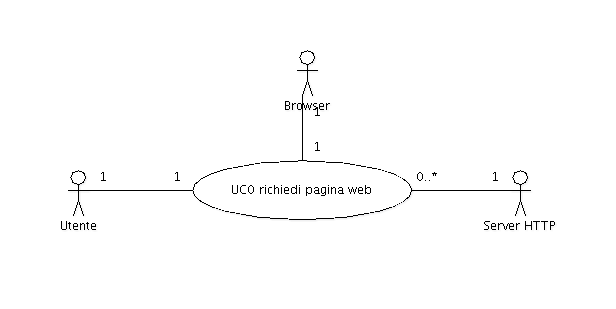
\includegraphics{UCAvvio.png}
\caption{Avvio dell'applicazione}
\end{figure}

Segue ora una descrizione testuale del caso d'uso presentato dal grafico.

\subsubsezione{UC0 Caso d'uso: richiedi pagina web}
\paragraph{Attori coinvolti} Utente, browser, server HTTP.
\paragraph{Scopo e descrizione sintetica}
L'utente avvia l'applicazione visualizzandone la relativa pagina web attraverso il browser, che richiede la relativa pagina al server HTTP.
\paragraph{Flusso di eventi}
\begin{elenconumerato}[\textbf{}]{\subsubsecindent}
\item L'utente inserisce l'URL relativo all'applicazione nel browser.
\item Il browser richiede la pagina al server HTTP.
\item Il server HTTP invia la pagina.
\item Il browser visualizza la pagina.
\end{elenconumerato}
\paragraph{Flusso alternativo}
Se viene rilevato un browser non supportato, l'utente viene avvisato. L'utente pu\`o decidere di continuare ugualmente senza nessuna garanzia di corretto funzionamento.
\paragraph{Precondizioni} Il browser \`e avviato. \`E possibile connettersi al server.
\paragraph{Postcondizioni} L'applicazione \`e avviata.

\subsezione{Interazione con l'applicazione}
Il seguente grafico descrive le interazioni tra l'utente finale e l'applicazione da un punto di vista ad alto livello. Le interazioni principali verranno poi espanse.
\begin{figure}[!ht]
\centering
\vspace{20pt} 
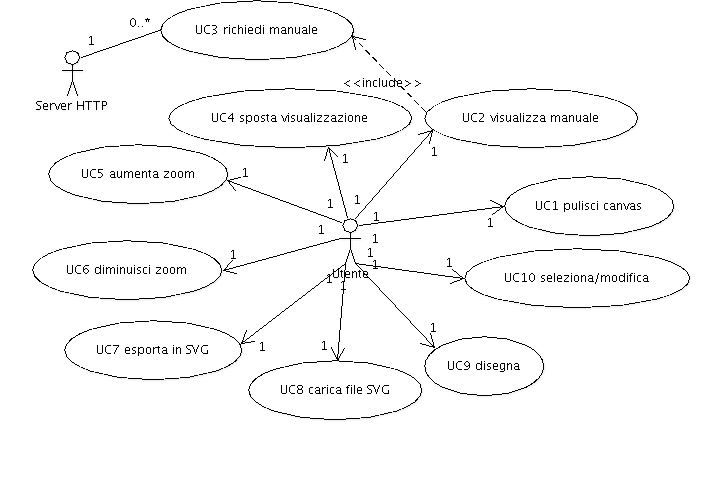
\includegraphics{UCInterazione.png}
\caption{Funzionalit\`a dell'applicazione}
\end{figure}

\text{Segue ora una descrizione testuale dei casi d'uso presentati dal grafico.}

\subsubsezione{UC1 Caso d'uso: pulisci \underline{canvas}}
\paragraph{Attori coinvolti} Utente.
\paragraph{Scopo e descrizione sintetica}
L'utente pu\`o cancellare totalmente quanto fino a quel momento \`e stato disegnato.
\paragraph{Flusso di eventi}
\begin{elenconumerato}[\textbf{}]{\subsubsecindent}
\item L'utente seleziona il comando per pulire il canvas. 
\item Il canvas viene completamente cancellato.
\end{elenconumerato}
\paragraph{Precondizioni} Il canvas \`e visibile.
\paragraph{Postcondizioni} Il canvas \`e vuoto.

\subsubsezione{UC2 Caso d'uso: visualizza manuale}
\paragraph{Attori coinvolti} Utente.
\paragraph{Scopo e descrizione sintetica}
L'utente pu\`o visualizzare il manuale dell'applicazione in linea.
\paragraph{Flusso di eventi}
\begin{elenconumerato}[\textbf{}]{\subsubsecindent}
\item L'utente seleziona il comando per visualizzare il manuale. 
\item Il manuale viene visualizzato mediante l'apertura di una nuova pagina HTML.
\end{elenconumerato}
\paragraph{Precondizioni} Il manuale utente non \`e visualizzato.
\paragraph{Postcondizioni} Il manuale utente \`e visualizzato.

\subsubsezione{UC3 Caso d'uso: richiedi manuale}
\paragraph{Attori coinvolti} Server HTTP.
\paragraph{Scopo e descrizione sintetica}
La/le pagina/e web contenenti il manuale utente sono gestite dal server HTTP.
\paragraph{Flusso di eventi}
\begin{elenconumerato}[\textbf{}]{\subsubsecindent}
\item Il sistema richiede la pagina web contenente il manuale utente al server HTTP.
\item Il server HTTP ritorna la pagina richiesta.
\end{elenconumerato}
\paragraph{Flusso alternativo}
Se il server HTTP non \`e disponibile o vi \`e un errore di comunicazione, l'utente viene avvisato.
\paragraph{Precondizioni} L'utente ha richiesto al sistema la visualizzazione del manuale o di parte di esso. \`E possibile connettersi al server.
\paragraph{Postcondizioni} Il sistema dispone del manuale.

\subsubsezione{UC4 Caso d'uso: sposta visualizzazione}
\paragraph{Attori coinvolti} Utente.
\paragraph{Scopo e descrizione sintetica}
Quando il canvas appare troppo grande per essere completamente visualizzato, l'utente pu\`o spostare la visualizzazione per scorrerne le sue diverse parti.
\paragraph{Flusso di eventi}
\begin{elenconumerato}[\textbf{}]{\subsubsecindent}
\item L'utente seleziona la parte del canvas da visualizzare.
\item Il sistema visualizza la parte di canvas selezionata al centro dello schermo.
\end{elenconumerato}
\paragraph{Precondizioni} Il canvas non \`e completamente visualizzato a schermo.
\paragraph{Postcondizioni} L'utente vede su schermo la parte di canvas desiderata.

\subsubsezione{UC5 Caso d'uso: aumenta livello di zoom}
\paragraph{Attori coinvolti} Utente.
\paragraph{Scopo e descrizione sintetica} 
Il sistema permette all'utente di ingrandire il canvas ed il suo contenuto mantendendo le proporzioni.
\paragraph{Flusso di eventi}
\begin{elenconumerato}[\textbf{}]{\subsubsecindent}
\item L'utente seleziona, esplicitamente o implicitamente, la parte di canvas da mantenere al centro della visualizzazione.
\item L'utente sceglie di quale percentuale aumentare lo zoom.
\item Il sistema ingrandisce il canvas di quanto richiesto.
\item Il sistema centra la visualizzazione nel punto richiesto dall'utente.
\end{elenconumerato}
\paragraph{Precondizioni} Il canvas \`e visualizzato.
\paragraph{Postcondizioni} Il canvas \`e ingrandito nel punto selezionato.

\subsubsezione{UC6 Caso d'uso: diminuisci zoom}
\paragraph{Attori coinvolti} Utente.
\paragraph{Scopo e descrizione sintetica} 
Il sistema permette all'utente di rimpicciolire il canvas ed il suo contenuto mantendendo le proporzioni.
\paragraph{Flusso di eventi}
\begin{elenconumerato}[\textbf{}]{\subsubsecindent}
\item L'utente seleziona, esplicitamente o implicitamente, la parte di canvas da mantenere al centro della visualizzazione.
\item L'utente sceglie di quale percentuale diminuire lo zoom.
\item Il sistema rimpicciolisce il canvas di quanto richiesto.
\item Il sistema accentra la visualizzazione dove richiesto dall'utente.
\end{elenconumerato}
\paragraph{Precondizioni} Il canvas \`e visualizzato.
\paragraph{Postcondizioni} Il canvas \`e rimpicciolito nel punto selezionato.

\subsubsezione{UC7 Caso d'uso: esporta in SVG}
\paragraph{Attori coinvolti} Utente.
\paragraph{Scopo e descrizione sintetica} 
Il sistema permette all'utente di esportare in formato di immagine SVG il contenuto del canvas.
\paragraph{Flusso di eventi}
\begin{elenconumerato}[\textbf{}]{\subsubsecindent}
\item L'utente seleziona il comando per esportare il canvas in formato SVG.
\item Il sistema genera un file SVG il cui contenuto corrisponde a quanto correntemente visualizzato nel canvas.
\item Il sistema rende disponibile all'utente il file generato.
\end{elenconumerato}
\paragraph{Precondizioni} Il canvas \`e visualizzato.
\paragraph{Postcondizioni} Il file SVG \`e disponibile all'utente e contiene quanto visualizzato nel canvas.

\subsubsezione{UC8 Caso d'uso: carica file SVG}
\paragraph{Attori coinvolti} Utente.
\paragraph{Scopo e descrizione sintetica} 
Il sistema permette all'utente di caricare file in formato SVG nel canvas.
\paragraph{Flusso di eventi}
\begin{elenconumerato}[\textbf{}]{\subsubsecindent}
\item L'utente seleziona il comando per caricare il file SVG.
\item L'utente seleziona il file SVG.
\item Il sistema visualizza il file SVG nel canvas. Se il file contiene elementi o attributi non supportati, essi saranno ignorati.
\end{elenconumerato}
\paragraph{Flusso alternativo}
Se il file non pu\`o essere caricato a causa di un errore in lettura o perch\`e non \`e un file SVG, l'utente verr\`a avvisato dell'errore e l'applicazione ritorner\`a allo stato precedente l'esecuzione del comando.
\paragraph{Precondizioni} Il canvas \`e visualizzato.
\paragraph{Postcondizioni} Il canvas contiene la visualizzazione del file SVG selezionato dall'utente ed \`e modificabile.

\subsubsezione{UC9 Caso d'uso: disegna}
Si rimanda a \ref{ucdisegna} per una descrizione approfondita.

\subsubsezione{UC10 Caso d'uso: seleziona e modifica}
Si rimanda a \ref{ucselezionaemodifica} per una descrizione approfondita.
\newpage
\subsezione{Vista UC9 - Disegna}
\label{ucdisegna}
Il seguente grafico illustra le interazioni tra l'utente e il sistema per disegnare un oggetto sul canvas.

\begin{figure}[!ht]
\centering
\vspace{20pt} 
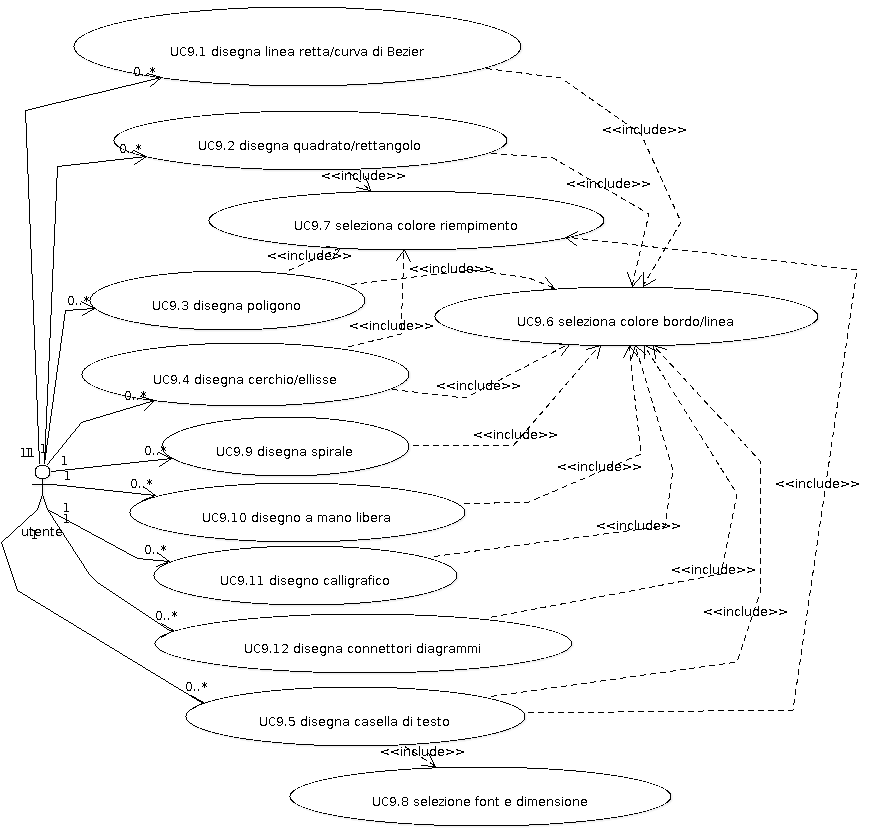
\includegraphics{UC9Espanso}
\caption{UC9 Caso d'uso: disegna}
\label{uc9}
\end{figure}


\subsubsezione{UC9.1 Caso d'uso: disegna linea retta/curva di Bezier}
\paragraph{Attori coinvolti} Utente.
\paragraph{Scopo e descrizione sintetica} 
Il sistema permette all'utente di disegnare una linea retta o una curva di Bezier.
\paragraph{Flusso di eventi}
\begin{elenconumerato}[\textbf{}]{\subsubsecindent}
\item L'utente seleziona il comando per disegnare una linea retta o una curva di Bezier.
\item L'utente disegna sul canvas la linea retta con due clic distinti, oppure la curva di Bezier tenendo premuto il pulsante sinistro del mouse.
\item Il sistema disegna la linea/curva.
\end{elenconumerato}
\paragraph{Precondizioni} Il canvas \`e visualizzato.
\paragraph{Postcondizioni} Il canvas mostra la nuova retta/curva disegnata.

\subsubsezione{UC9.2 Caso d'uso: disegna quadrato/rettangolo}
\paragraph{Attori coinvolti} Utente.
\paragraph{Scopo e descrizione sintetica} 
Il sistema permette all'utente di disegnare un quadrato o un rettangolo di qualsiasi dimensione.
\paragraph{Flusso di eventi}
\begin{elenconumerato}[\textbf{}]{\subsubsecindent}
\item L'utente seleziona il comando per disegnare un quadrato o un rettangolo.
\item L'utente disegna sul canvas il quadrato o il rettangolo, regolando col cursore la sua dimensione.
\item Il sistema disegna il quadrato/rettangolo.
\end{elenconumerato}
\paragraph{Precondizioni} Il canvas \`e visualizzato.
\paragraph{Postcondizioni} Il canvas mostra il nuovo quadrato/rettangolo disegnato.

\subsubsezione{UC9.3 Caso d'uso: disegna poligono}
\paragraph{Attori coinvolti} Utente.
\paragraph{Scopo e descrizione sintetica} 
Il sistema permette all'utente di disegnare un poligono di qualsiasi dimensione e numero di vertici.
\paragraph{Flusso di eventi}
\begin{elenconumerato}[\textbf{}]{\subsubsecindent}
\item L'utente seleziona il comando per disegnare un poligono.
\item L'utente seleziona il numero di vertici del poligono che intende disegnare.
\item L'utente disegna sul canvas il poligono, regolando col cursore la sua dimensione.
\item Il sistema disegna il poligono.
\end{elenconumerato}
\paragraph{Precondizioni} Il canvas \`e visualizzato.
\paragraph{Postcondizioni} Il canvas mostra il nuovo poligono disegnato.

\subsubsezione{UC9.4 Caso d'uso: disegna cerchio/ellisse}
\paragraph{Attori coinvolti} Utente.
\paragraph{Scopo e descrizione sintetica} 
Il sistema permette all'utente di disegnare un cerchio o un'ellisse di qualsiasi dimensione.
\paragraph{Flusso di eventi}
\begin{elenconumerato}[\textbf{}]{\subsubsecindent}
\item L'utente seleziona il comando per disegnare un cerchio o un'ellisse.
\item L'utente disegna sul canvas il cerchio o l'ellisse, regolando col cursore la sua dimensione.
\item Il sistema disegna il cerchio o l'ellisse.
\end{elenconumerato}
\paragraph{Precondizioni} Il canvas \`e visualizzato.
\paragraph{Postcondizioni} Il canvas mostra il nuovo cerchio o la nuova ellisse disegnato/a.

\subsubsezione{UC9.5 Caso d'uso: disegna casella di testo}
\paragraph{Attori coinvolti} Utente.
\paragraph{Scopo e descrizione sintetica} 
Il sistema permette all'utente di disegnare una casella di testo.
\paragraph{Flusso di eventi}
\begin{elenconumerato}[\textbf{}]{\subsubsecindent}
\item L'utente seleziona il comando per disegnare una casella di testo.
\item L'utente disegna sul canvas la casella, regolando col cursore la sua dimensione.
\item L'utente scrive il testo all'interno della casella.
\item Il sistema disegna la casella di testo.
\end{elenconumerato}
\paragraph{Precondizioni} Il canvas \`e visualizzato.
\paragraph{Postcondizioni} Il canvas mostra la nuova casella di testo disegnata.

\subsubsezione{UC9.6 Caso d'uso: seleziona colore bordo/linea}
\paragraph{Attori coinvolti} Utente.
\paragraph{Scopo e descrizione sintetica} 
Il sistema permette all'utente di selezionare il colore del bordo della figura da disegnare, oppure del testo da scrivere.
\paragraph{Flusso di eventi}
\begin{elenconumerato}[\textbf{}]{\subsubsecindent}
\item L'utente seleziona il colore dalla paletta.
\item Il sistema imposta il colore dato dall'utente come base per la figura da disegnare.
\end{elenconumerato}
\paragraph{Precondizioni} Il canvas \`e visualizzato.
\paragraph{Postcondizioni} Il canvas \`e visualizzato. La prossima figura verr\` a disegnata con il colore del bordo selezionato.

\subsubsezione{UC9.7 Caso d'uso: seleziona colore riempimento}
\paragraph{Attori coinvolti} Utente.
\paragraph{Scopo e descrizione sintetica} 
Il sistema permette all'utente di selezionare il colore di riempimento del poligono da disegnare.
\paragraph{Flusso di eventi}
\begin{elenconumerato}[\textbf{}]{\subsubsecindent}
\item L'utente seleziona il colore di riempimento del poligono dalla paletta.
\item Il sistema imposta il colore dato dall'utente come base per la figura da disegnare.
\end{elenconumerato}
\paragraph{Precondizioni} Il canvas \`e visualizzato.
\paragraph{Postcondizioni} Il canvas \`e visualizzato. La prossima figura verr\` a disegnata con il colore di riempimento selezionato.

\subsubsezione{UC9.8 Caso d'uso: selezione font e dimensione carattere}
\paragraph{Attori coinvolti} Utente.
\paragraph{Scopo e descrizione sintetica} 
Il sistema permette all'utente di selezionare il tipo e la dimensione del carattere da disegnare.
\paragraph{Flusso di eventi}
\begin{elenconumerato}[\textbf{}]{\subsubsecindent}
\item L'utente seleziona il tipo di carattere e la sua dimensione.
\item Il sistema imposta i valori dati dall'utente come base per la prossima casella di testo da disegnare.
\end{elenconumerato}
\paragraph{Precondizioni} Il canvas \`e visualizzato.
\paragraph{Postcondizioni} Il canvas \`e visualizzato. La prossima casella di testo verr\` a disegnata con i parametri selezionati.

\subsubsezione{UC9.9 Caso d'uso: disegna spirale}
\paragraph{Attori coinvolti} Utente.
\paragraph{Scopo e descrizione sintetica} 
Il sistema permette all'utente di disegnare una spirale.
\paragraph{Flusso di eventi}
\begin{elenconumerato}[\textbf{}]{\subsubsecindent}
\item L'utente seleziona il comando per disegnare una spirale.
\item L'utente disegna la spirale sul canvas, regolando col cursore la sua ampiezza.
\item Il sistema disegna la spirale.
\end{elenconumerato}
\paragraph{Precondizioni} Il canvas \`e visualizzato.
\paragraph{Postcondizioni} Il canvas mostra la nuova spirale disegnata.

\subsubsezione{UC9.10 Caso d'uso: disegno di linee a mano libera}
\paragraph{Attori coinvolti} Utente.
\paragraph{Scopo e descrizione sintetica} 
Il sistema permette all'utente di disegnare linee a mano libera.
\paragraph{Flusso di eventi}
\begin{elenconumerato}[\textbf{}]{\subsubsecindent}
\item L'utente seleziona il comando per disegnare linee a mano libera.
\item L'utente disegna la linea a mano libera sul canvas, trascinando il cursore.
\item Il sistema disegna la linea creata.
\end{elenconumerato}
\paragraph{Precondizioni} Il canvas \`e visualizzato.
\paragraph{Postcondizioni} Il canvas mostra la nuova linea a mano libera.

\subsubsezione{UC9.11 Caso d'uso: disegno calligrafico}
\paragraph{Attori coinvolti} Utente.
\paragraph{Scopo e descrizione sintetica} 
Il sistema permette all'utente di creare linee calligrafiche che emulano l'azione dell'inchiostro su carta.
\paragraph{Flusso di eventi}
\begin{elenconumerato}[\textbf{}]{\subsubsecindent}
\item L'utente seleziona il comando per disegnare linee calligrafiche.
\item L'utente disegna la linea calligrafica sul canvas, trascinando il cursore.
\item Il sistema disegna la linea creata.
\end{elenconumerato}
\paragraph{Precondizioni} Il canvas \`e visualizzato.
\paragraph{Postcondizioni} Il canvas mostra la nuova linea calligrafica.

\subsubsezione{UC9.12 Caso d'uso: disegno connettori di diagrammi}
\paragraph{Attori coinvolti} Utente.
\paragraph{Scopo e descrizione sintetica} 
Il sistema permette all'utente di disegnare dei connettori di diagrammi.
\paragraph{Flusso di eventi}
\begin{elenconumerato}[\textbf{}]{\subsubsecindent}
\item L'utente seleziona il comando per disegnare connettori di diagrammi.
\item L'utente disegna il connettore sul canvas, cliccando su punto d'inizio e punto di fine linea desiderati.
\item Il sistema disegna il connettore creato.
\end{elenconumerato}
\paragraph{Precondizioni} Il canvas \`e visualizzato.
\paragraph{Postcondizioni} Il canvas mostra il nuovo connettore creato.
\newpage
\subsezione{Vista UC10 - Seleziona e Modifica}
\label{ucselezionaemodifica}
Il seguente grafico illustra le interazioni tra l'utente e il sistema per selezionare e modificare un oggetto sul canvas.

\begin{figure}[!ht]
\centering
\vspace{20pt} 
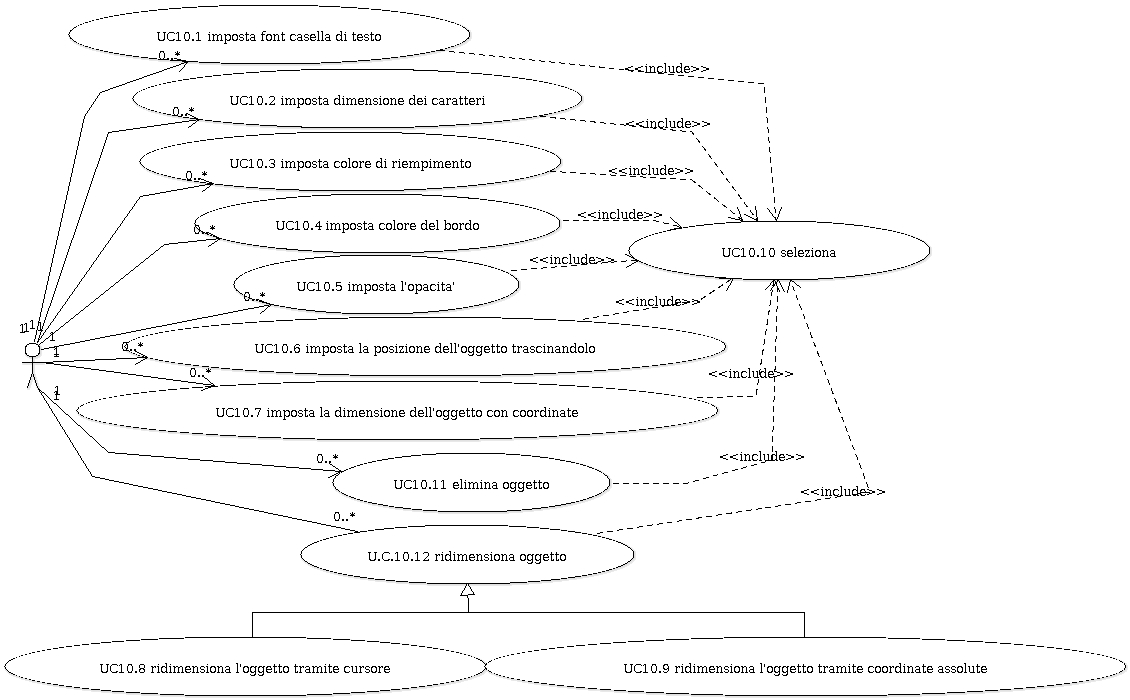
\includegraphics{UC10Espanso.jpg}
\caption{UC10 Caso d'uso: seleziona e modifica}
\label{uc10}
\end{figure}
\newpage
\subsubsezione{UC10.1 Caso d'uso: imposta font casella di testo}
\paragraph{Attori coinvolti} Utente.
\paragraph{Scopo e descrizione sintetica} 
Il sistema consente all'utente di impostare il font del testo presente all'interno di una casella di testo.
\paragraph{Flusso di eventi}
\begin{elenconumerato}[\textbf{}]{\subsubsecindent}
\item L'utente seleziona una casella di testo.
\item Il sistema evidenzia l'etichetta di testo selezionata e mostra un pannello con i relativi stili grafici.
\item L'utente porta il cursore nella sezione/scheda del pannello relativa al font.
\item L'utente seleziona il font scelto all'interno di tale pannello.
\end{elenconumerato}
\paragraph{Precondizioni} L'utente ha scelto una casella di testo presente nel canvas.
\paragraph{Postcondizioni} Le propriet\` a degli stili grafici della casella di testo indicano che il font usato \` e quello selezionato (la casella potrebbe essere vuota e quindi non visibile dall'utente all'interno del canvas).

\subsubsezione{UC10.2 Caso d'uso: imposta dimensione dei caratteri}
\paragraph{Attori coinvolti} Utente.
\paragraph{Scopo e descrizione sintetica} 
Il sistema consente di modificare la dimensione dei caratteri del testo di una casella.
\paragraph{Flusso di eventi}
\begin{elenconumerato}[\textbf{}]{\subsubsecindent}
\item L'utente seleziona una casella di testo.
\item Il sistema evidenzia l'etichetta di testo selezionata e mostra un pannello con i relativi stili grafici.
\item L'utente porta il cursore nella sezione/scheda del pannello relativa alla dimensione carattere.
\item L'utente seleziona la dimensione scelta nel combobox apposito all'interno di tale pannello, o inserisce un numero intero valido.
\end{elenconumerato}
\paragraph{Precondizioni}L'utente ha scelto una casella di testo presente nel canvas.
\paragraph{Postcondizioni}Le propriet\`a degli stili grafici della casella di testo indicano che la dimensione del font \` e quella selezionata (parte del testo potrebbe essere troncata o non visibile).

\subsubsezione{UC10.3  Caso d'uso: imposta colore di riempimento}
\paragraph{Attori coinvolti} Utente.
\paragraph{Scopo e descrizione sintetica}   Il sistema consente di personalizzare il colore dello spazio appartenente ad un qualsiasi oggetto presente nel canvas. Sono disponibili colori campione, e colori personalizzati (mixando le componenti \underline{RGB} che producono il corrispondente codice esadecimale del colore a 6 cifre).
\paragraph{Flusso di eventi}
\begin{elenconumerato}[\textbf{}]{\subsubsecindent}
\item L'utente seleziona un oggetto valido.
\item Il sistema evidenzia l'oggetto selezionato e mostra un pannello con i relativi stili grafici.
\item L'utente porta il cursore nella sezione/scheda del pannello relativa al colore di riempimento.
\item L'utente seleziona un colore nel menu a tendina apposito all'interno di tale pannello (caso colore campione).
\item L'utente si reca nel menu a tendina apposito all'interno di tale pannello. Clicca sulla scheda alternativa e mixa il colore impostando i valori rosso, blu, verde (caso colore personalizzato).
\end{elenconumerato}
\paragraph{Precondizioni}L'utente ha scelto un oggetto colorabile presente nel canvas.
\paragraph{Postcondizioni}Le propriet\` a degli stili grafici della casella di testo indicano che il colore di riempimento \` e  quello selezionato (il colore potrebbe essere uguale allo sfondo del canvas e quindi non visibile dall'utente).


\subsubsezione{UC10.4  Caso d'uso: imposta colore del bordo}
\paragraph{Attori coinvolti} Utente.
\paragraph{Scopo e descrizione sintetica} Il sistema consente di personalizzare il colore di tutto il bordo appartenente ad un qualsiasi oggetto presente nel canvas. Sono disponibili colori campione, e colori personalizzati (mixando le componenti RGB che producono il corrispondente codice esadecimale del colore a 6 cifre).
\paragraph{Flusso di eventi}
\begin{elenconumerato}[\textbf{}]{\subsubsecindent}
\item L'utente seleziona un oggetto valido.
\item Il sistema evidenzia l'oggetto selezionato e mostra un pannello con i relativi stili grafici.
\item L'utente  porta  il cursore nella sezione/scheda del pannello relativa al colore del bordo.
\item L'utente seleziona un colore  nel menu a tendina apposito all'interno di tale pannello(caso colore campione).
\item L'utente si reca nel menu a tendina apposito all'interno di tale pannello. Clicca sulla scheda alternativa e mixa il colore impostando i valori rosso, blu, verde (caso colore personalizzato).
\end{elenconumerato}
\paragraph{Precondizioni} L'utente ha scelto un oggetto colorabile presente nel canvas.
\paragraph{Postcondizioni} Le propriet\` a degli stili grafici della casella di testo indicano che il colore del bordo \`e quello selezionato (il colore potrebbe essere uguale allo sfondo del canvas e quindi il bordo potrebbe diventare non visibile dall'utente).


\subsubsezione{UC10.5  Caso d'uso: imposta l'opacit\` a}
\paragraph{Attori coinvolti} Utente.
\paragraph{Scopo e descrizione sintetica}  Il sistema consente di modificare il livello di opacit\` a di un qualsiasi oggetto presente nel canvas. Il valore si esprime in \%.   \` E quindi possibile rendere un oggetto pienamente visibile (100\%), non visibile (0\%), e situazioni intermedie.
\paragraph{Flusso di eventi}
\begin{elenconumerato}[\textbf{}]{\subsubsecindent}
\item L'utente seleziona un oggetto valido.
\item Il sistema evidenzia l'oggetto selezionato e mostra un pannello con i relativi stili grafici.
\item L'utente porta  il cursore nella sezione/scheda del pannello relativa all'opacit\` a.
\item L'utente regola l'opacit\` a inserendo un valore intero compreso tra 0 e 100 oppure trascinando col cursore l'apposito mixer.
\end{elenconumerato}
\paragraph{Precondizioni} L'utente ha scelto un oggetto presente nel canvas.
\paragraph{Postcondizioni} Le propriet\` a degli stili grafici della casella di testo indicano che l'opacit\` a dell'oggetto corrisponde al valore intero selezionato.

\subsubsezione{UC10.6   Caso d'uso: imposta la posizione trascinando l'oggetto}
\paragraph{Attori coinvolti} Utente.
\paragraph{Scopo e descrizione sintetica} Il sistema consente di modificare la posizione di un qualsiasi oggetto presente nel canvas. L'utente utilizza il cursore per trascinare l'oggetto dove desidera.
\paragraph{Flusso di eventi}
\begin{elenconumerato}[\textbf{}]{\subsubsecindent}
\item L'utente seleziona una oggetto valido.
\item Il sistema evidenzia l'oggetto selezionato e mostra un pannello con i relativi stili grafici.
\item L'utente trascina l'oggetto in una posizione valida all'interno dell'area del canvas usando il cursore.
\end{elenconumerato}
\paragraph{Precondizioni} L'utente ha scelto un oggetto presente nel canvas. L'utente non pu\` o trascinare l'oggetto fuori dal canvas.
\paragraph{Postcondizioni} Le propriet\` a degli stili grafici della casella di testo indicano che l'oggetto \` e nella nuova posizione. Il canvas visualizza l'oggetto nella nuova posizione.
 

\subsubsezione{UC10.7 Caso d'uso: imposta la posizione dell'oggetto tramite coordinate}
\paragraph{Attori coinvolti} Utente.
\paragraph{Scopo e descrizione sintetica}   Il sistema consente di modificare la posizione di un qualsiasi oggetto tramite coordinate.  L'utente  imposta la posizione in modo assoluto. Ogni oggetto infatti, di qualsiasi forma esso sia, occupa un'area rettangolare. La posizione di tale area \`e descritta da quattro valori interi che rappresentano le coordinate dei suoi vertici significativi. I primi due interi per ordinata/ascissa del vertice in alto a sinistra. Il terzo e quarto valore rispettivamente per ordinata/ascissa del vertice in basso a destra.
\paragraph{Flusso di eventi}
\begin{elenconumerato}[\textbf{}]{\subsubsecindent}
\item  L'utente seleziona un oggetto valido.
\item  Il sistema evidenzia l'oggetto selezionato e mostra un pannello con i relativi stili grafici.
\item  L'utente porta  il cursore nella sezione/scheda del pannello relativa alla dimensione dell'oggetto.
\item  L'utente imposta manualmente i quattro valori della dimensione dell'oggetto.
\end{elenconumerato}
\paragraph{Precondizioni} L'utente ha scelto un oggetto  presente nel canvas. Se l'utente sceglie una posizione non valida (che porterebbe l'oggetto ad uscire dal canvas) il sistema posiziona l'oggetto nel valore valido pi\` u vicino a quello selezionato (ad esempio sul bordo estremo del canvas). Valori negativi vengono ignorati.
\paragraph{Postcondizioni} Le propriet\`  a degli stili grafici della casella di testo indicano che l'oggetto \`e nella nuova posizione. Il canvas visualizza l'oggetto nella nuova posizione.

\subsubsezione{UC10.8 Caso d'uso: ridimensiona l'oggetto tramite cursore}
\paragraph{Attori coinvolti} Utente.
\paragraph{Scopo e descrizione sintetica}  Il sistema consente di modificare le dimensioni  di un qualsiasi oggetto presente nel canvas.  L'utente utilizza il cursore per ingrandire / rimpicciolire a piacere l'oggetto.
\paragraph{Flusso di eventi}
\begin{elenconumerato}[\textbf{}]{\subsubsecindent}
\item  L'utente seleziona un oggetto valido.
\item  Il sistema evidenzia l'oggetto selezionato e mostra un pannello con i relativi stili grafici.
\item  L'utente usa il cursore con puntatore specifico per modificare le dimensioni dell'oggetto.
\end{elenconumerato}
\paragraph{Precondizioni} L'utente ha scelto un oggetto presente nel canvas. Se le dimensioni sono superiori a un valore massimo relativo della dimensione del canvas, il sistema le imposta alla massima dimensione consentita.
\paragraph{Postcondizioni} Le propriet\`a  degli stili grafici della casella di testo indicano che le dimensioni dell'oggetto sono quelle selezionate. L'oggetto si ingrandir\` a/rimpicciolir\`a  a seconda dei movimenti del cursore.


\subsubsezione{UC10.9 Caso d'uso: ridimensiona l'oggetto tramite coordinate assolute}
\paragraph{Attori coinvolti} Utente.
\paragraph{Scopo e descrizione sintetica} Il sistema consente di modificare le dimensioni  di un qualsiasi oggetto presente nel canvas tramite l'inserimento di coordinate assolute.  Ogni oggetto, di qualsiasi forma esso sia, occupa un area rettangolare. Quindi ogni oggetto possiede due valori interi che rappresentano le due dimensioni (base, altezza). Quadrato e cerchio presentano solo un unica dimensione.
\paragraph{Flusso di eventi}
\begin{elenconumerato}[\textbf{}]{\subsubsecindent}
\item  L'utente seleziona un oggetto valido.
\item  Il sistema evidenzia l'oggetto selezionato e mostra un pannello con i relativi stili grafici.
\item  L'utente porta il cursore nella sezione/scheda del pannello relativa alla dimensione dell'oggetto.
\item  L'utente imposta manualmente i due valori della dimensione dell'oggetto.
(base e altezza). Nel caso di cerchio e quadrato  \`e  presente un solo intero da impostare (dimensione unica).
\end{elenconumerato}
\paragraph{Precondizioni} L'utente ha scelto un oggetto presente nel canvas. Non si accettano valori negativi o pari a zero. Se le dimensioni sono superiori a un massimo relativo alla dimensione del canvas il sistema le imposta alla massima dimensione consentita.
\paragraph{Postcondizioni} Le propriet\` a degli stili grafici della casella di testo indicano che le dimensioni dell'oggetto  sono quelle selezionate. L'oggetto si ingrandir\`a/rimpicciolir\`a  a seconda dei valori interi inseriti.
                   
\subsubsezione{UC10.10 Caso d'uso: seleziona}
\paragraph{Attori coinvolti} Utente.
\paragraph{Scopo e descrizione sintetica} Il sistema consente di selezionare un qualsiasi oggetto presente nel canvas.
\paragraph{Flusso di eventi}
\begin{elenconumerato}[\textbf{}]{\subsubsecindent}
\item  L'utente seleziona il comando per la selezione di un oggetto.
\item  L'utente usa il cursore per selezionare l'oggetto in questione.
\end{elenconumerato}
\paragraph{Precondizioni} Il canvas \`e visualizzato. L'utente ha selezionato un oggetto presente nel canvas.
\paragraph{Postcondizioni} Il sistema evidenzia l'oggetto selezionato e mostra un pannello con i relativi stili grafici.

\subsubsezione{UC10.11 Caso d'uso: elimina oggetto}
\paragraph{Attori coinvolti} Utente.
\paragraph{Scopo e descrizione sintetica} Il sistema consente di eliminare dal canvas un qualsiasi oggetto.
\paragraph{Flusso di eventi}
\begin{elenconumerato}[\textbf{}]{\subsubsecindent}
\item  L'utente seleziona il comando per la selezione di un oggetto.
\item  L'utente usa il cursore per selezionare l'oggetto in questione.
\item  L'utente seleziona il comando per la cancellazione di un oggetto.
\end{elenconumerato}
\paragraph{Precondizioni} Il canvas \`e visualizzato. L'utente ha selezionato un oggetto presente nel canvas.
\paragraph{Postcondizioni} Il canvas non visualizza l'oggetto cancellato.


%%%%%%%%%%%%%%%%inizio requisiti%%%%%%%%%%%%%%%%%%%%%%%%%%%%%%%
\sezione{Lista dei requisiti}
\label{listarequisiti}
I requisiti elencati in seguito si dividono per tipologia (funzionale, prestazionale, di qualit\`a, di interfacciamento, d'ambiente); 
per ognuna \`e presente una classificazione per classe di importanza (obbligatorio, desiderabile, facoltativo). Viene inoltre indicata la fonte usando un riferimento alle aspettative descritte in \textit{Aspettative.pdf}.
\subsezione{Requisiti funzionali (RF)}
\subsubsezione{Obbligatori (RFO)}
\begin{elenconumerato}[\textbf{RFO-}]{\subsubsecindent}
\item{ACO-2 - AJAXDRAW permette di disegnare linee rette.}
\item{ACO-2 - AJAXDRAW permette di disegnare curve di Bezier.}
\item{ACO-2 - AJAXDRAW permette di disegnare quadrilateri di qualsiasi dimensione(quadrata o rettangolare).}
\item{ACO-2 - AJAXDRAW permette di disegnare poligoni regolari di qualsiasi dimensione e numero di lati.}
\item{ACO-2 - AJAXDRAW permette all'utente di disegnare cerchi o ellissi.}
\item{ACO-2 - AJAXDRAW permette di aggiungere caselle di testo al documento. }
\item{ACO-2 - AJAXDRAW permette la modifica del font e della dimensione del testo presente nelle caselle disegnate.}
\item{ACO-2, ACO-3 - Per ogni elemento disegnato, AJAXDRAW permette all'utente di selezionare e spostare tale elemento.}
\item{ACO-3 - AJAXDRAW permette di cambiare il colore di riempimento, del bordo, delle linee, dell'opacit\`a degli oggetti disegnati.}
\item{ACO-3 - AJAXDRAW permette il ridimensionamento degli oggetti disegnati.}
\item{ACO-2 - AJAXDRAW permette all'utente di selezionare ognuna delle funzionalit\`a suddette tramite una comoda barra degli strumenti.}
\item{ACO-2 - Qualora suddette funzioni siano regolate da parametri, AJAXDRAW permette all'utente di impostarli.}
\item {ACO-2 - Qualora il canvas risulti troppo grande per essere mostrato completamente su schermo, l'utente pu\`o spostare la visualizzazione per scorrerne le sue diverse parti.}
\item{ACO-2 - AJAXDRAW permette di effettuare uno zoom in avanti e all'indietro nel disegno.}
\item{ACO-4 - AJAXDRAW \`e in grado di salvare le immagini create dall'utente nel formato SVG.}
\item{ACO-4 - AJAXDRAW permette di caricare immagini in formato SVG che utilizzano il sottoinsieme che AJAXDRAW \`e in grado di generare.}
\end{elenconumerato}

%requisiti desiderabili
\subsubsezione{Desiderabili (RFD)}
\begin{elenconumerato}[\textbf{RFD-}]{\subsubsecindent}
\item{ACF-2 - AJAXDRAW permette di disegnare a mano libera.}
\item{ACF-2 - AJAXDRAW permette di disegnare connettori per diagrammi.}
\item{ACF-1 - AJAXDRAW permette di cancellare completamente l'area di disegno.}
\item{ACF-1 - AJAXDRAW permette di cancellare un singolo oggetto disegnato.}
\end{elenconumerato}

%facoltativi
\subsubsezione{Facoltativi (RFF)}
\begin{elenconumerato}[\textbf{RFF-}]{\subsubsecindent}
\item{ACF-2 - AJAXDRAW permette la creazione di spirali.}
\item{ACF-2 - AJAXDRAW permette di utilizzare il disegno calligrafico o pennellato.}
\end{elenconumerato}

%requisiti prestazionali
\subsezione{Requisiti prestazionali}
\subsubsezione{Obbligatori (RPO)}
\begin{elenconumerato}[\textbf{RPO-}]{\subsubsecindent}
\item ACO-1 - L'utente non deve notare rallentamenti durante l'utilizzo dell'applicazione che non siano direttamente imputabili alla lentezza della connessione.
\end{elenconumerato}

%Requisiti di Qualità
\subsezione{Requisiti di qualit\`a (RQ)}	
\subsubsezione{Obbligatori (RQO)}
\begin{elenconumerato}[\textbf{RQO-}]{\subsubsecindent}
\item ACO-5 - Il lato client dell'applicativo dev'essere realizzato usando tecnologie web standard
\footnote{con il termine \H{}standard\H{} si intendono tecnologie effettivamente standardizzate come l'\underline{ECMAScript} o tecnologie considerate standard \textit{de facto} come quelle raccomandata dal \textit{W3C}.}
\item ACO-8 - Il codice sorgente segue le norme interne all'azienda.
\item ACO-8 - Il codice sorgente segue il paradigma della programmazione ad oggetti.
\item ACO-8 - Il codice sorgente \`e completamente documentato.
\item ACO-8 - La progettazione permetter\`a l'estensibilit\`a futura del prodotto.
\item ACO-8 - I test del prodotto saranno documentati.
\item ACO-5 - Il prodotto non necessita di nessuna installazione, basandosi su una pagina web HTML.
\item ACO-5 - Il server dev'essere in grado di gestire pi\`u utenti in parallelo in modo indipendente.
\item ACO-1 - Il funzionamento dell'applicazione dev'essere indipendente dalla risoluzione dello schermo dell'utente.
\end{elenconumerato}

%requisiti di qualita' desiderabili
%\subsubsezione{Desiderabili (RQD)}
%\begin{elenconumerato}[\textbf{RQD-}]{\subsubsecindent}
%\item 

%\end{elenconumerato}

%inizio requisiti di interfacciamento
\subsezione{Requisiti di interfacciamento (RI)}
\subsubsezione{Obbligatori (RIO)}
\begin{elenconumerato}[\textbf{RIO-}]{\subsubsecindent}
\item ACO-7 - L'utilizzo del prodotto risulta semplice ed intuitivo grazie ad un'interfaccia grafica basata sull'uso di una toolbar.
\item ACO-7 - La guida in linea \`e completa e di facile utilizzo per permettere all'utente di apprendere velocemente le funzionalit\`a del prodotto.
\item ACO-7 - La guida in linea \`e richiamabile in qualsiasi momento.
\item ACO-7 - L'uso della guida in linea non influenza il corretto funzionamento del programma. 
\end{elenconumerato}

%inizio requisiti d'ambiente
\subsezione{Requisiti d'ambiente (RA)}
\subsubsezione{Obbligatori (RAO)}
\begin{elenconumerato}[\textbf{RAO-}]{\subsubsecindent}
\item ACO-5 - Il prodotto \`e pensato per funzionare su un internet browser.
\item ACO-5 - Il prodotto dovr\`a essere implementato seguendo gli standard del \underline{linguaggio di markup} HTML 5.
\item ACO-6 - Il prodotto in particolare dovr\` a utilizzare il tag "canvas" appositamente creato per l'elaborazione del disegno vettoriale sul web.
\item ACO-8 - Il software di supporto per lo sviluppo del prodotto \`e di tipo Open Source e freeware.
\item ACD-1 - Il prodotto realizzato dovr\`a essere pubblicato sul sito \href{www.sourceforge.net}{www.sourceforge.net}, in conformit\`a con i relativi requisiti di natura Open Source, per favorire la continuit\`a del prodotto risultante.
\item ACO-5 - Il prodotto \`e sviluppato e testato sui principali internet browsers: Mozilla Firefox, Google Chrome, Opera ed Apple Safari.
\end{elenconumerato}
\subsubsezione{Desiderabili (RAD)}
\begin{elenconumerato}[\textbf{RAD-}]{\subsubsecindent}
\item{ACF-3 - AJAXDRAW garantisce la compatibilit\`a con il browser Microsoft Internet Explorer, il quale non implementa a pieno HTML 5, tramite la libreria \H{}excanvas\H{} creata da Google.}
\end{elenconumerato}

\newpage

 \subsezione{Tracciamento Requisiti - Use Case}
\begin{table}[h]
\begin{center}
     \begin{tabular}
           {@{\extracolsep{\fill}}|c|c|}
     \hline
%%%%%%%%%%%%%%INTESTAZIONE COLONNE%%%%%%%%%%%%%%%%%%%%%%%%%%%%%%%%
      \textbf{Requisiti} & \textbf{Use Case} \\
%%%%%%%%%%%%%%FINE INTESTAZIONE COLONNE%%%%%%%%%%%%%%%%%%%%%%%%%%%%%%%%%%%%%
      \hline
     RA0-1 & UC0 \\
     \hline
     RFD-3 & UC1  \\
     \hline
     RIO-2  RIO-4 & UC2\\
     \hline
     RIO-3 & UC3 \\
     \hline
     RFO-13 & UC4 \\
     \hline
     RFO-14 & UC5 UC6 \\
      \hline
     RFO-15 RFO-16 & UC7 UC8 \\
     \hline
     RFO-1 RFO-2 RFO-9 & UC9.1 \\
     \hline
     RFO-3 RFO-9 &  UC9.2 \\
     \hline
     RFO-4 RFO-9 & UC9.3 \\
     \hline
     RFO-5 RFO-9 & UC9.4 \\
     \hline
     RFO-6 RFO-7 RFO-9 & UC9.5 \\
     \hline
     RFO-9 & UC9.6 UC9.7 \\
     \hline
     RFF-1 RFO-9 & UC9.9 \\
     \hline
     RFD-1 RFO-9 & UC9.10 \\
     \hline
     RFF-2 RFO-9 & UC9.11 \\
     \hline 
     RFD-2 RFO-9 & UC9.12 \\
     \hline
     RFO-7 & UC 9.8 UC10.1 UC10.2 \\
     \hline
     RFO-9 & UC10.3 UC10.4 UC10.5 \\
     \hline
     RFO-8 & UC10.5 UC10.7 UC10.10 \\
     \hline
     RFO-10 & UC10.8 UC10.9 \\
     \hline
     RFD-4 & UC10.11 \\
     
%%%%%%%%%%% PARTE DA MODIFICARE %%%%%%%%%%%%%%%%
    \hline %%FINE RIGA
%%%%%%%%%%% FINE PARTE DA MODIFICARE %%%%%%%%%%%%%%%%%%%%%%%%%%%%%%%%%%%%%%%%
    \end{tabular}
  \caption{Requisiti - Use Case} %INSERIRE DIDASCALIA - SE NECESSARIA -
  \label{tab:requisiti}
  \end{center}
\end{table}
\end{document}